\chapter{Choix du matériel et du logiciel}
\label{Chapitre:Choix du Hardware et du Software}
\thispagestyle{fancy}

\section{Méthodes d'enregistrement d'un signal EEG}
\label{Section:3.Méthodes d'enregistrement d'un signal EEG}

Il existe deux types de systèmes électroencéphalographiques :
\smallbreak
\begin{itemize}
	\item \textbf{Les EEG intracrâniens}. Il s'agit de systèmes dits invasifs : on vient enregistrer l'activité neuronale du cerveau en implantant des électrodes directement dans la boite crânienne. Bien que cette technique offre des résultats probants, elle nécessite une intervention chirurgicale, ce qui n'est pas réalisable dans le cadre de notre projet. 
	\smallbreak
	\item \textbf{Les EEG de scalpe (ou de surface)}. Ce système étudie les variations du courant diffusé par le cerveau sur la surface du crâne. Il s'agit d'un système non invasif et c'est en toute logique que nous utiliserons ce type de dispositif.

\end{itemize}
\smallbreak
La visualisation et l'enregistrement d'un signal EEG passe donc par l'utilisation d'électrodes. Il s'agit de capteurs sensibles aux variations du champ électrique générées par les échanges électriques entre les neurones. Le signal EEG est atténué par des éléments physiques comme le crâne ou la peau, il doit donc être amplifié afin d'être visualisé et traité. Du bruit est également observé lors de l'acquisition de signaux EEG. Celui-ci provient à la fois du cerveau et de l'environnement extérieur. 

\begin{figure}[h]
	\centering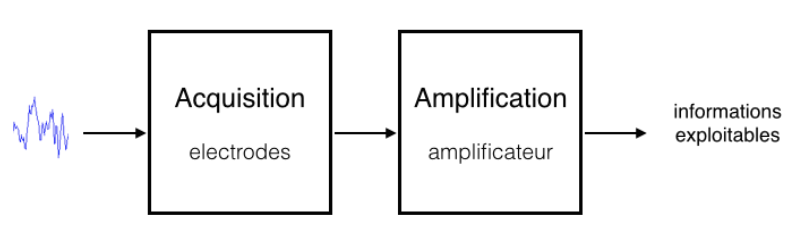
\includegraphics[width=14cm]{images/chaineSignal.png}
	\caption{Chaine d'acquisition d'un signal EEG}
	\label{fig:GRASS}
\end{figure}

\section{Caractéristiques générales du matériel}
\label{Section:3.Caractéristiques générales du matériel}

\subsection{Électrodes}
\label{Subsection:3.Électrodes}

Il existe différents types d'électrodes :
\smallbreak
\begin{itemize}
	\item \textbf{Les électrodes jetables}.
	\smallbreak 
	\subitem - \textbf{Les électrodes sèches.} Se sont les plus simples à utiliser car elles ne nécessitent pas l'utilisation de gel pour réaliser le contact avec la peau. Elles sont cependant moins précises que des électrodes à gel.
	\smallbreak
	\subitem - \textbf{Les électrodes à gel}. Ce type d'électrode utilise un gel afin d'améliorer le contact entre l'électrode et la surface du crâne.  
	\smallbreak
	\item \textbf{Les électrodes réutilisables}. Elles sont constituées de matériaux conducteurs permettant de capter les courants présents. Différents matériaux peuvent être utilisés (or, acier inoxydable, argent, etc.), chacun possédant une qualité de conduction plus ou moins élevée. 
	\smallbreak
	\item \textbf{Les casques à électrodes}. Ce sont les dispositifs les plus utilisés en R\&D. Ils offrent une stabilité accrue vis à vis du placement des électrodes et évitent ainsi l'introduction de bruits.
	\smallbreak
	\item \textbf{Les électrodes à aiguilles}. Il s'agit d'électrodes possédant une partie sous-cutanée. Elles offrent de bons résultats mais la pose nécessite l'assistance d'un médecin.
\end{itemize}
\smallbreak
Après étude des avantages et des inconvénients des différents systèmes, notre choix se porte sur l'utilisation d'un casque à électrodes. 

Plus le nombre d'électrodes utilisées est élevé, plus la qualité de l'information spatiale sera importante. Le placement des électrodes de surface au niveau de la boîte crânienne répond au standard "International 10-20 System" (Figure \ref{fig:InternationalSystem}). Chaque zone du cerveau est donc scrutée par une électrode. On parle alors de canal. (exemple : O1 correspond au canal analysant par la partie occipitale gauche du cortex, O2 la partie droite).

\begin{figure}[h]
	\centering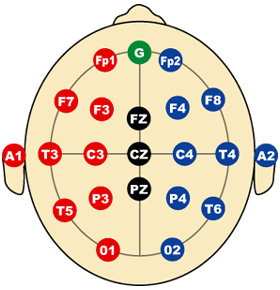
\includegraphics[width=6cm]{images/electrodesStandard.png}
	\caption[Standard International 10-20 System à 23 électrodes.]{Standard International 10-20 System à 23 électrodes\\Source : https://tel.archives-ouvertes.fr/tel-00822833/document}
	\label{fig:InternationalSystem}
\end{figure}

\subsection{Amplificateur}
\label{Subsection:3.Amplificateur}

L'amplificateur effectue deux tâches : l'amplification des signaux EEG et leur échantillonnage. Certains amplificateurs proposent également de réaliser un filtrage temporel. Nous souhaitons cependant l'implémenter par nos propres moyens dans ce projet. Un amplificateur est caractérisé par : 
\smallbreak
\begin{itemize}
	\item Son gain.
	\smallbreak
	\item Son taux d'échantillonnage.
	\smallbreak
	\item Sa résolution numérique.
	\smallbreak
	\item Son ratio signal sur bruit. 
\end{itemize}
\smallbreak
Il existe des amplificateurs directement intégrés dans le casque EEG, cependant leur qualité reste moindre que les systèmes conventionnels. Leur usage est principalement destiné aux jeux vidéos et n'est pas adapté à la réalisation d'examens médicaux. 

\section {Choix du matériel}
\label{Section:3.Choix du matériel}
Pour ce projet, nous disposons du matériel suivant :
\smallbreak
\begin{itemize}
	\item Le casque biopac CAP100C, composé de 19 électrodes à gel \cite{biopac} (Figure \ref{fig:CAP100C}).
	\smallbreak
	\item L'amplificateur 15LT de Grass Technologies. Il s'agit d'un amplificateur de 16 canaux. Il est utilisable à la fois pour les EEG, les EMG et les ECG. Celui-ci est fournit avec un logiciel propriétaire, GrassLab, permettant l'acquisition et l'exportation des données \cite{grass} (Figure \ref{Grass}).
\end{itemize}

\smallbreak

\begin{figure}[h]
	\centering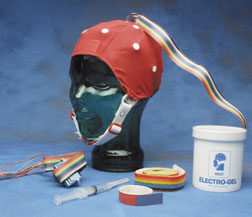
\includegraphics[width=7cm]{images/cap100.jpg}
	\caption[CAP100C de Biopac]{CAP100C de Biopac.\\Source : http://www.biopac.com/BioNomadix-EEG-CAP-medium}
	\label{fig:CAP100C}
\end{figure}

\begin{figure}[h]
	\centering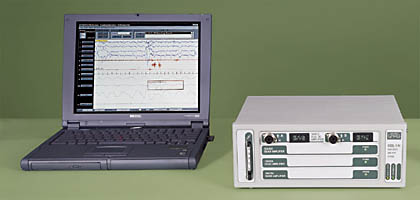
\includegraphics[width=10cm]{images/GRASS.jpg}
	\caption[GRASS amplifier 15LT]{GRASS amplifier 15LT.\\Source : http://www.grasstechnologies.com/products/ampsystems/15lt.html}
	\label{Grass}
\end{figure}

Pour commencer, nous avons utilisé le CAP100C de Biopac avec l'amplificateur GRASS. Nous avons pu observer les différents signaux EEG (concentration, calcul mental simple, repos, lecture, etc). Notre objectif étant de réaliser une interface cerveau-ordinateur dans un cadre pédagogique, ce matériel ne semble pas adapté pour plusieurs raisons :
\smallbreak
\begin{itemize}
	\item Casque et amplificateur Grass onéreux (difficile d'en avoir plusieurs exemplaires)
	\smallbreak
	\item Logiciel propriétaire GrassLab obsolète, le support technique n'est plus assuré.
	\smallbreak
	\item Confort d'utilisation du casque discutable.
	\smallbreak
	\item Le produit s'adresse essentiellement au marché médical.
\end{itemize}
On souhaite acquérir un autre système EEG plus adapté à l'utilisation dans le cadre d'un cours. Une étude comparative de différents produits du marché est proposée (Voir le tableau présenté en annexe). D'après l'analyse comparative, notre choix se porte sur la gamme de produit de la marque Emotiv. En effet, le prix des produits est attractif pour les performances proposées, et est cohérent avec notre budget. Voici un tableau qui présente les principales différences entre les 3 casques de la marque.

\begin{figure}[h]
	\centering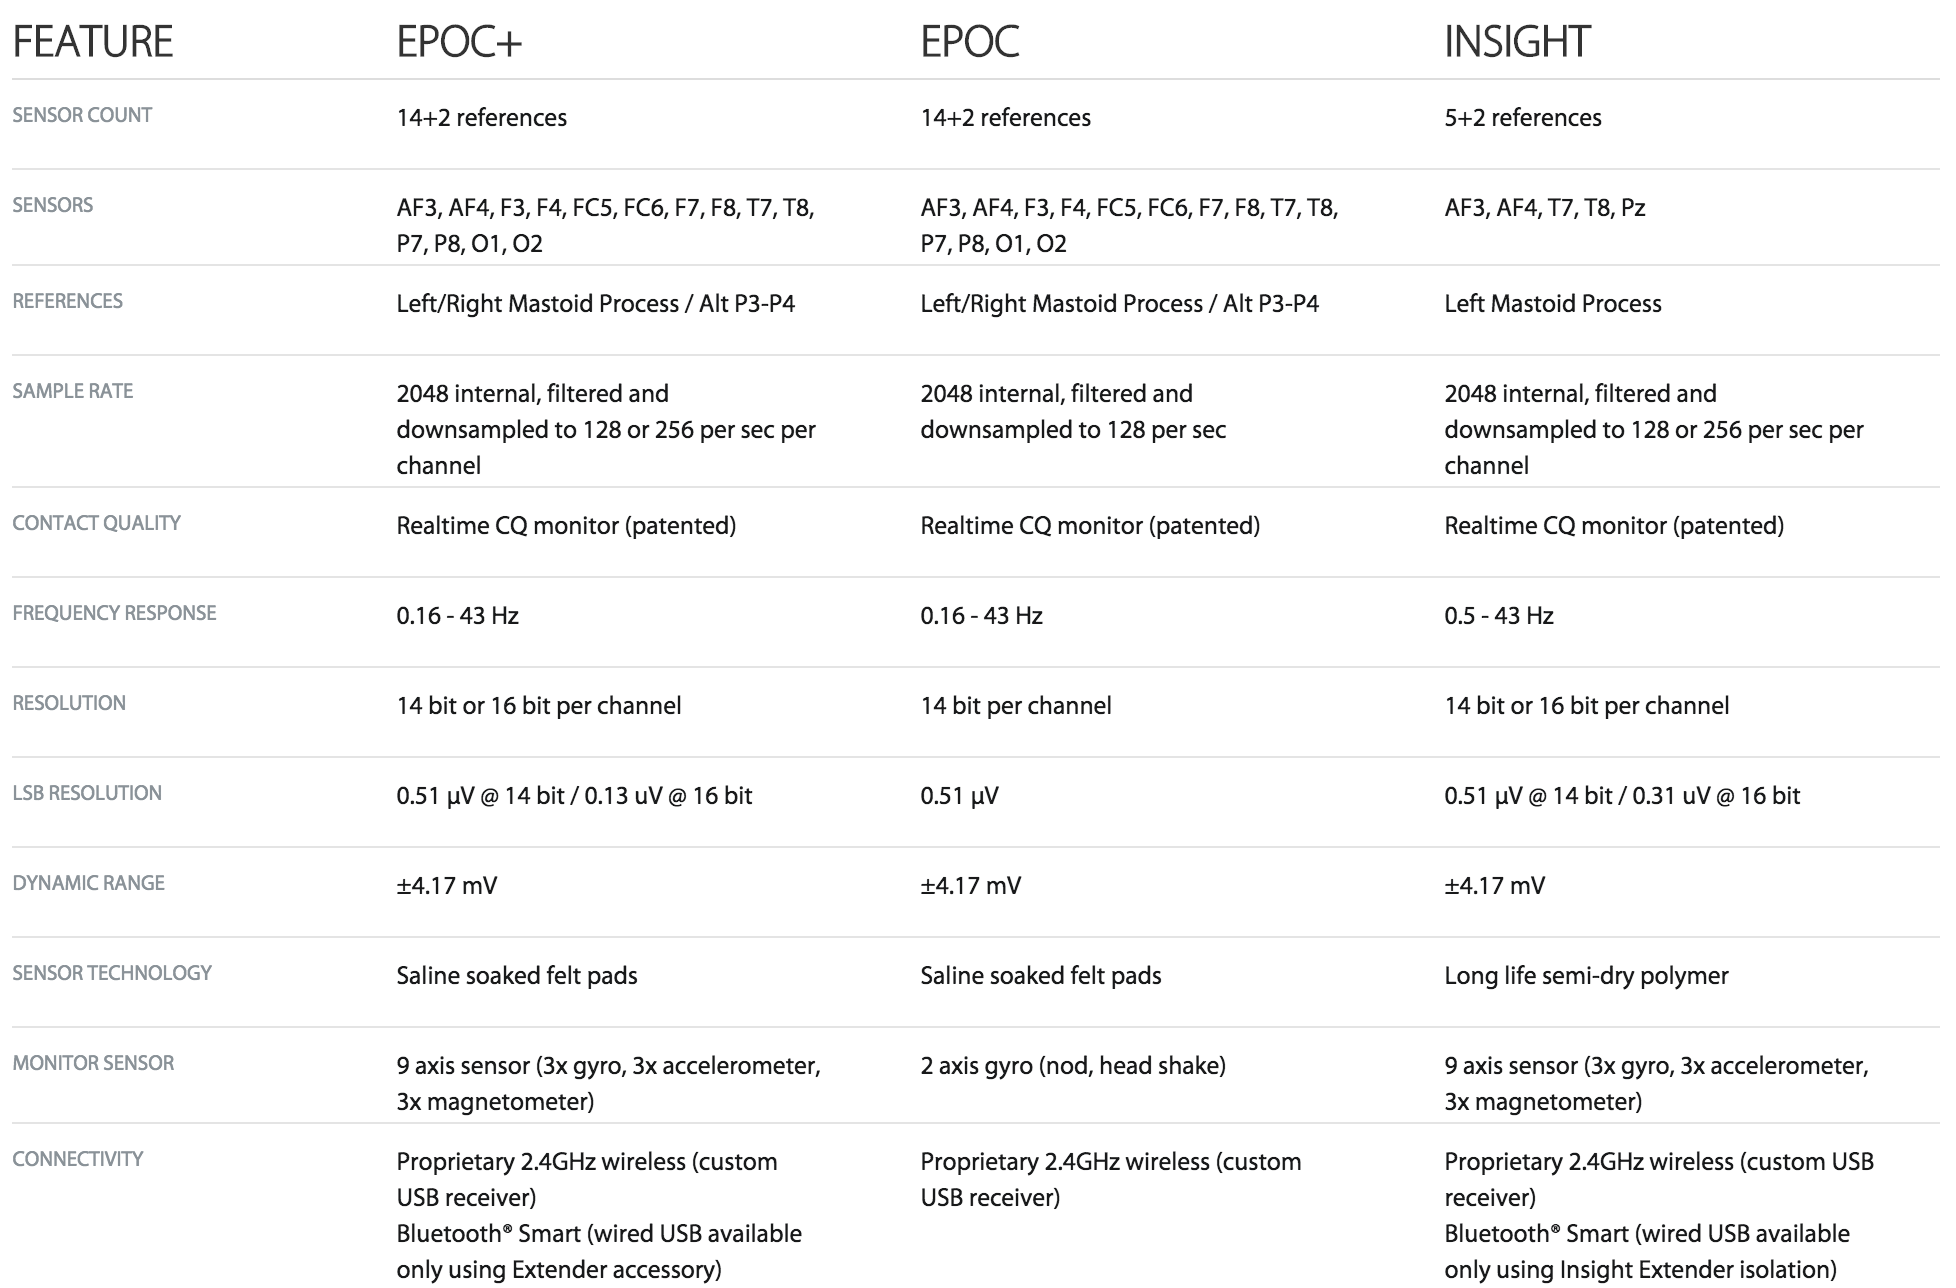
\includegraphics[width=15cm,height=15cm]{images/emotiv_comparaison.png}
	\caption[Comparaison entre les différents casques Emotiv]{Comparaison entre les différents casques Emotiv \\Source : http://emotiv.com}
	\label{fig:Emotiv_Comparaison}
\end{figure}

Le casque Emotiv INSIGHT n'est pas assez performant pour nos travaux et convient plus pour des activités vidéoludiques (iI ne dispose que de 5 capteurs). En revanche, les casques EPOC et EPOC+ semblent plus adaptés \cite{epoc}. Il est possible d'accéder aux données EEG brutes, à condition d'acquérir une licence SDK. 
Après étude des produits, nous proposons à l'université de Sherbrooke d'acquérir le casque EPOC.
 Voici le devis : 
\begin{itemize}
	\smallbreak
	\item Casque : 399\$US;
	\smallbreak
	\item SDK "licence de recherche individuelle" : 300\$US.
	\smallbreak
	\item Licence supplémentaire Mac OS X : 90 \$US.
	\smallbreak
	\item Total : 789\$US.
\end{itemize}

\begin{figure}[h]
	\centering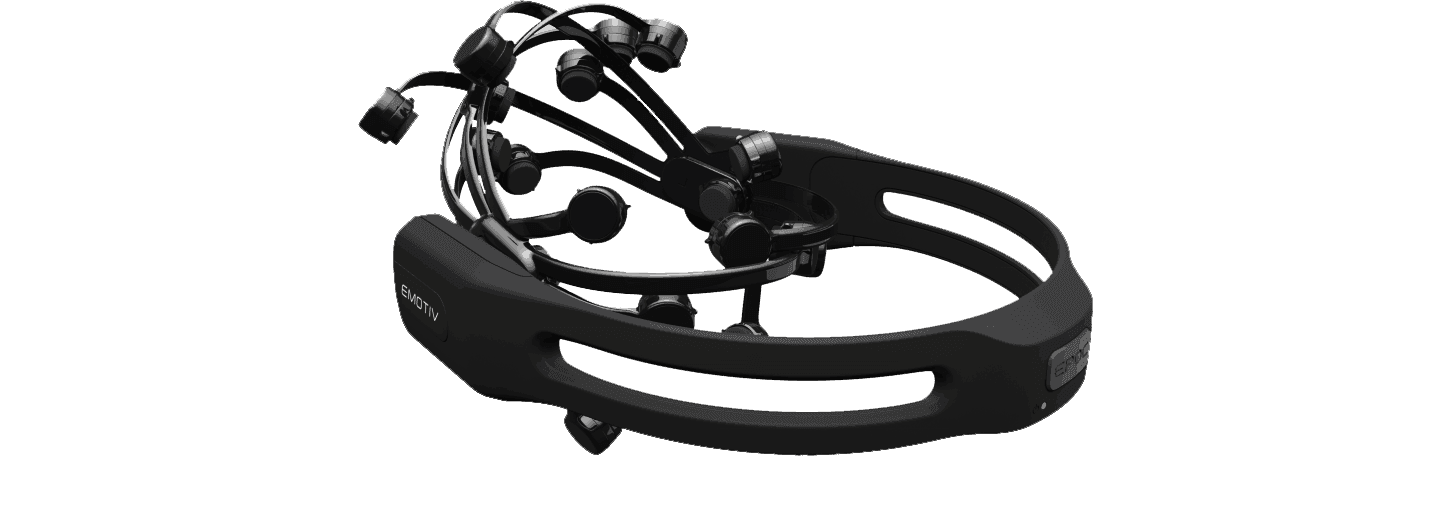
\includegraphics[width=12cm]{images/EPOC.png}
	\caption[EPOC headset - Emotiv]{EPOC headset - Emotiv.\\ Source : http://emotiv.com}
	\label{fig:EPOC}
\end{figure}

\section {Choix du logiciel}
\label{Section:3.Choix du logiciel}
Il existe principalement deux logiciels libres de droit, compatibles avec le casque EPOC : EEGLAB et OpenViBE (Open Virtual Brain Environment).
\smallbreak
EEGLAB fonctionne avec l'outil Simulink de Matlab. Il est majoritairement utilisé pour le traitement du signal. Il nécessite cependant l'acquisition d'une licence Matlab pour chaque poste de travail, ce qui peut s'avérer onéreux dans le cadre d'un cours suivi par plusieurs étudiants.
\smallbreak
OpenVIBE propose quant à lui sa propre interface (i.e. fonctionne sans logiciel tiers). Il est majoritairement utilisé dans le développement de liaisons cerveau-ordinateur. Celui-ci est gratuit, fonctionnel avec le casque EPOC, bien documenté et performant. Il fonctionne de plus sur les plateformes Windows et Linux. Ce logiciel a été développé par l'équipe de l'Institut National de Recherche en Informatique et Automatique (INRIA) de Rennes en France.